\documentclass[a4paper,12pt]{article}

\usepackage[utf8]{inputenc}
\usepackage[T1]{fontenc}
\usepackage[czech]{babel}
\usepackage[scaled]{helvet}
\renewcommand{\familydefault}{\sfdefault}
\usepackage{graphicx}
\usepackage{hyperref}
\usepackage{geometry}
\usepackage{booktabs}
\usepackage{float}
\usepackage{wrapfig}
\usepackage{fancyhdr}
\usepackage{qrcode}
\usepackage{xcolor}

\geometry{margin=1cm, top=2.5cm, headheight=1.5cm, headsep=0.3cm}

\pagestyle{fancy}
\fancyhf{}
\fancyhead[L]{
\includegraphics[height=1.2cm]{obrazky/UREL_logo.pdf}}
\fancyhead[C]{{\Huge\textbf{\textit{Semafor}}}}
\fancyhead[R]{{\begingroup\hypersetup{urlcolor=black}\qrcode[height=2cm]{https://github.com/fatalwir/Semafor/dokumentace/navod_semafor.pdf}\endgroup}}
\renewcommand{\headrulewidth}{0pt}

\hypersetup{
    colorlinks=true,
    linkcolor=blue,
    urlcolor=blue,
}

\title{Semafor návod}
\author{Ing. Ondřej Kolář}
\date{\today}

\setcounter{secnumdepth}{0}

\begin{document}

\subsection{Popis zapojení}
drgdgdegrregt

\begin{center}
    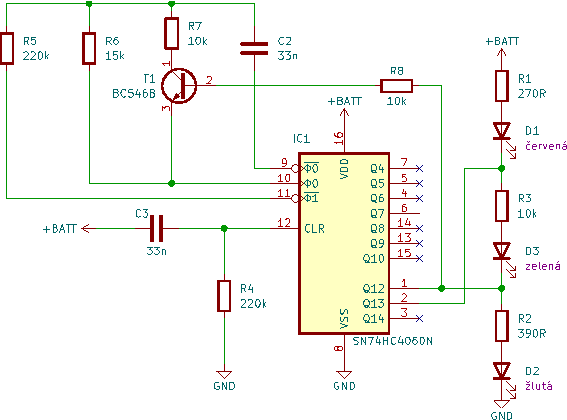
\includegraphics[width=.7\textwidth]{obrazky/schema_navod.pdf}
\end{center}


\subsection{Postup oživení}

\begin{wrapfigure}{r}{0.3\textwidth}
    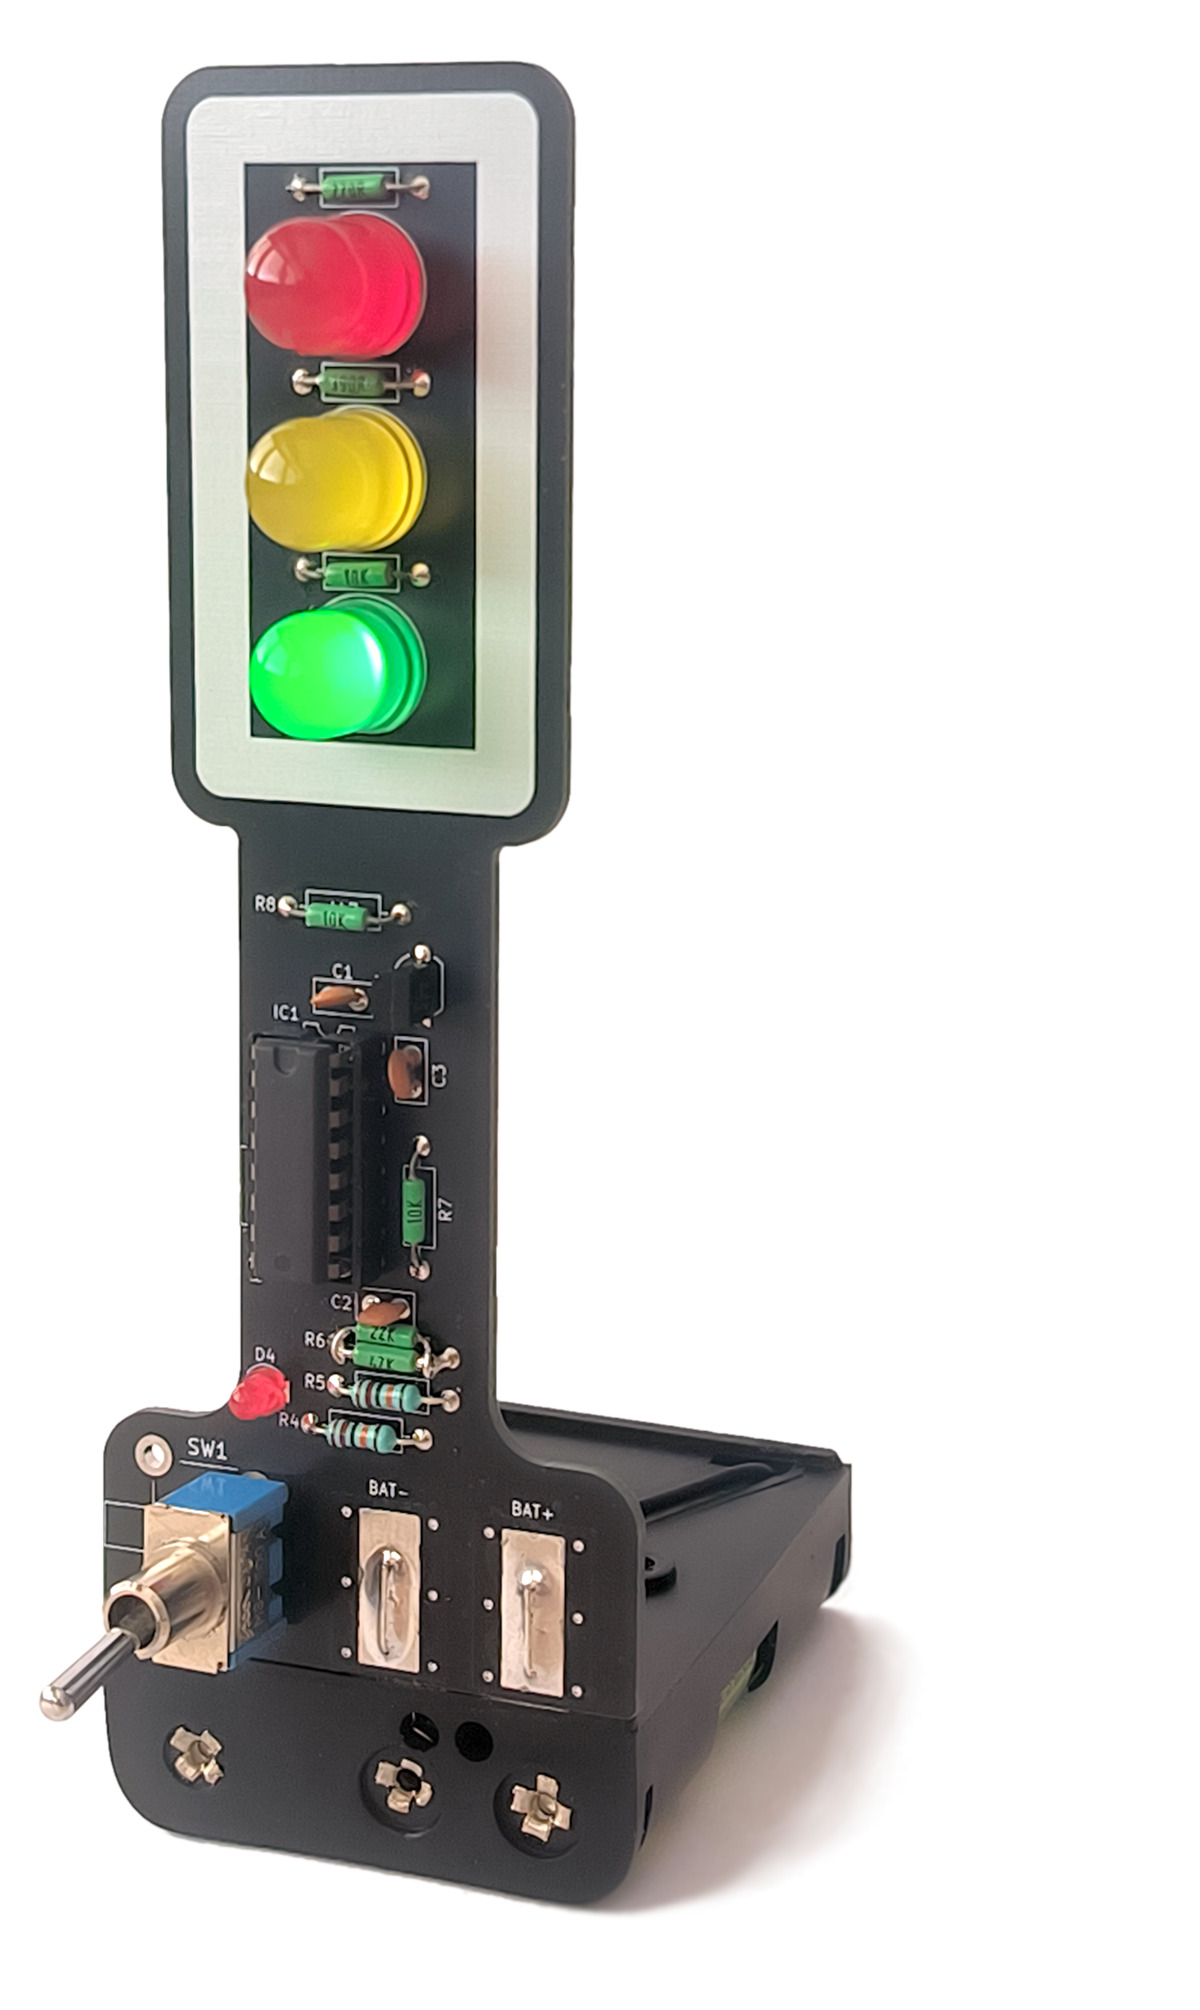
\includegraphics[width=0.3\textwidth]{obrazky/foto.jpg}
\end{wrapfigure}

Toto dílo je licencováno pod Standardní licencí pro digitální soubory
Digitální soubory mají přísnou nekomerční licenci pouze pro osobní použití.

Soubory nesmíte sdílet, poskytovat sublicence, prodávat, pronajímat, hostovat, přenášet nebo jakkoli distribuovat digitální soubor nebo 3D tištěnou verzi tohoto objektu, ani žádné jiné odvozené dílo tohoto objektu v digitálním nebo fyzickém formátu. (včetně remixů tohoto objektu)

Nesmíte tyto soubory hostovat na jiných digitálních platformách, webových obchodech nebo cloudových úložištích.
Objekty nesmíte bez povolení používat žádným způsobem, při kterém vybíráte peníze či poplatky.

\end{document}
